\colorlet{outlinecolor}{green}

\colorlet{headercolor}{outlinecolor}
\colorlet{rowcolor1}{outlinecolor!70}
\colorlet{rowcolor2}{outlinecolor!50}



\begin{tikzpicture}
	\node [mybox, fill=boxcolor, draw=outlinecolor] (box){%
		\begin{minipage}{0.3\textwidth}
			\vspace{0.1cm}
	
			\underline{Undo unwanted changes}: Once you've commited something, it's in Git forever. However, there are some things that can be undone.
			
			\vspace{-2mm}
			\begin{center}
					\textcolor{background}{
							\begin{tabularx}{\textwidth}{>{\columncolor{rowcolor1}}X|>{\columncolor{rowcolor2}}p{3.5cm}}
									\arrayrulecolor{boxcolor} % Table line color
									\rowcolor{headercolor} % Header row color
									\multicolumn{1}{c|}{\centering \textbf{Git Command}} & \multicolumn{1}{c}{\centering \textbf{Description}} \\ % Center the header text
									\hline % Add a horizontal line below the header row
									\rowcolor{rowcolor1} \tablebash{git reset HEAD your\_filename} & Undoes an unwanted \tablebash{git add} \\
									\rowcolor{rowcolor2} % Color of the second row
									\tablebash{git checkout -- your\_filename} & Reverts a file to its last commit version \\
									\rowcolor{rowcolor1} % New Row
									\tablebash{git commit --amend -m "new commit message"} & Update your Git commit message \\
								\end{tabularx}
						}
				\end{center}
		\end{minipage}
	};
	\node[fancytitle, right=10pt, fill=outlinecolor, text=background, draw=outlinecolor, rounded corners] at (box.north west) {Undo Unwanted Changes};
\end{tikzpicture}



\begin{tikzpicture}
	\node [mybox, fill=boxcolor, draw=outlinecolor] (box){%
		\begin{minipage}{0.3\textwidth}
			\vspace{0.1cm}
			
			\underline{Repo restructuring}: Here's how to get Git to track your repo structuring.
			
			\vspace{-2mm}
			\begin{center}
				\textcolor{background}{
					\begin{tabularx}{\textwidth}{>{\columncolor{rowcolor1}}X|>{\columncolor{rowcolor2}}p{4cm}}
						\arrayrulecolor{boxcolor} % Table line color
						\rowcolor{headercolor} % Header row color
						\multicolumn{1}{c|}{\centering \textbf{Git Command}} & \multicolumn{1}{c}{\centering \textbf{Description}} \\ % Center the header text
						\hline % Add a horizontal line below the header row
						\rowcolor{rowcolor1} \tablebash{git mv current\_filepath new\_filepath} & Rename your file and get Git to track it in one-go \\
						\rowcolor{rowcolor2} % New Row
						\tablebash{git rm your\_filename} & Simultaneously delete and stop tracking a file in one-go \\
						\rowcolor{rowcolor1} % Color of the second row
						\tablebash{git add -A} & Stages any file renaming or deletions done via your IDE \\
						\rowcolor{rowcolor2} % Color of the second row
						\tablebash{git checkout -- deleted\_filename} & Undo tracked file deletion \\
					\end{tabularx}
				}
			\end{center}
			
			%			\begin{minipage}{\textwidth}
				%				\centering
				%%				\vspace{-2mm}
				%				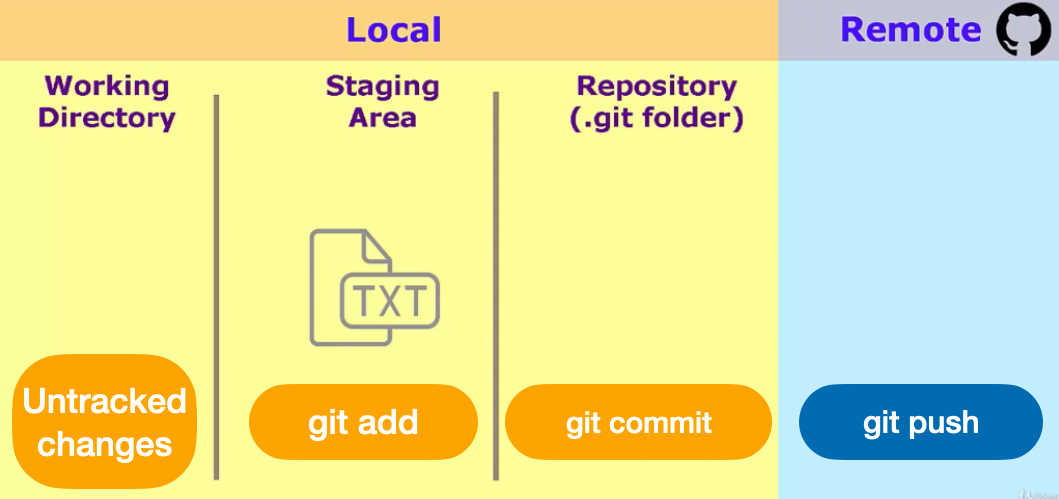
\includegraphics[width=0.5\textwidth]{images/git_stages.png}
				%				\vspace{-2mm}
				%				\captionof{figure}{Git states and associated commands. \href{https://www.udemy.com/course/git-complete/}{ \faLink{}  Source}}
				%			\end{minipage}
			
		\end{minipage}
	};
	\node[fancytitle, right=10pt, fill=outlinecolor, text=background, draw=outlinecolor, rounded corners] at (box.north west) {Track Wanted Changes};
\end{tikzpicture}
